\subsubsection{Tones}

You have probably heard that Chinese languages are tone languages, and know this means that sounds which are the same except for rise and fall of the voice mean different things. This somtimes leads to confusion and/or merriment when a foreigner gets a tone wrong in a phrase, and says 'lazy' when he means 'broken', 'sugar' when he means 'soup', 'ghost' when he means 'cupboard', and so on.

\tnote{The textbook uses 7 yale tones, but in jyutping there are only really 6. The 7 is going to be used to denote the examples in this section of the high falling tone, which in jyutping is now just 1 (high level).}

\begin{minipage}{\linewidth}
In Cantonese there are seven tones, that is seven variations in voice pitch having the power to combine with an otherwise identitcal syllable to make seven different meanings. This is best illustrated by examples, which your teacher will read to you:

\audioTag{A}{9:10}

\renewcommand{\arraystretch}{2}
\begin{tabularx}{\linewidth}{l l l r}
    \jping{si7} & 思 & think & (High falling tone) \\
    \jping{si2} & 史 & history & (High rising tone) \\
    \jping{si3} & 試 & try & (Mid level tone) \\
    \jping{si1} & 詩 & poem & (High level tone) \\
    \jping{si4} & 時 & time & (Low falling tone) \\
    \jping{si5} & 市 & market & (Low rising tone) \\
    \jping{si6} & 事 & a matter; business & (Low level tone) \\
\end{tabularx}
\renewcommand{\arraystretch}{1}
\end{minipage}

Below is a practice exercise on the seven tones. Close your books and concentrate on listening to the teacher or tape. Repeate loud and clear during the pause after each syllabe or group of sylables.

\audioTag{A}{9:27}

(This practice section on the basic tones was prepared by Prof. James E. Dew).

\todo{copy practice exercises}

%%%%%%%%%%%%%%%%%%%%%%%%%%%%%%%%%%%%%%%%
\begin{minipage}{\linewidth}

\paragraph{Discussion of Tones}

There are seven tones in Standard Cantonese. Their desginations together with examples of each tone, are:

\audioTag{A}{14:36}

\renewcommand{\arraystretch}{2}
\begin{tabularx}{\linewidth}{l l l l}
    \jping{si1} & 詩 & \jping{fan1} & 分 \\
    \jping{si7} & 思 & \jping{fan7} & 婚 \\
    \jping{si2} & 史 & \jping{fan2} & 粉 \\
    \jping{si3} & 試 & \jping{fan3} & 訓 \\
    \jping{si4} & 時 & \jping{fan4} & 墳 \\
    \jping{si5} & 市 & \jping{fan5} & 憤 \\
    \jping{si6} & 事 & \jping{fan6} & 份 \\
\end{tabularx}
\renewcommand{\arraystretch}{1}

You will note that the tones have three conotours - level, rising, and falling.

There are three level tones: high level, mid level, and low level.

\audioTag{A}{15:03}

\renewcommand{\arraystretch}{2}
\begin{tabularx}{\linewidth}{l l l}
    hl: & \jping{si1} & 詩 \\
    ml: & \jping{si3} & 試 \\
    ll: & \jping{si6} & 事 \\
\end{tabularx}
\renewcommand{\arraystretch}{1}

There are two rising tones: high rising and low rising.

\audioTag{A}{15:10}

\renewcommand{\arraystretch}{2}
\begin{tabularx}{\linewidth}{l l l}
    hr: & \jping{si2} & 史 \\
    lr: & \jping{si5} & 市 \\
\end{tabularx}
\renewcommand{\arraystretch}{1}

There are two falling tones: high falling and low falling.

\audioTag{A}{15:16}

\renewcommand{\arraystretch}{2}
\begin{tabularx}{\linewidth}{l l l l}
    hf: & \jping{si7} & 思 \\
    lf: & \jping{si4} & 時 \\
\end{tabularx}
\renewcommand{\arraystretch}{1}

\end{minipage}

\begin{minipage}{\linewidth}

Following a chart devised by Y. R. Chao, we graph the tones of Cantonese on a scale of one to five, thus:

\audioTag{A}{15:26}

\centering
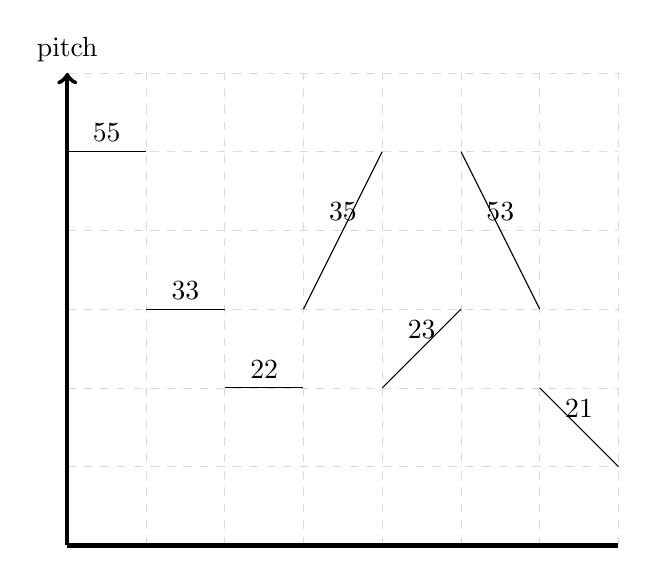
\begin{tikzpicture}
\draw [help lines, color=gray!30, dashed] (0, 0) grid (7, 6);
\draw [->, ultra thick] (0, 0) -- (0, 6) node [above]{pitch};
\draw [ultra thick] (0, 0) -- (7, 0);
\draw (0, 5) -- node [above]{55} (1, 5);
\draw (1, 3) -- node [above]{33} (2, 3);
\draw (2, 2) -- node [above]{22} (3, 2);
\draw (3, 3) -- node [above]{35} (4, 5);
\draw (4, 2) -- node [above]{23} (5, 3);
\draw (5, 5) -- node [above]{53} (6, 3);
\draw (6, 2) -- node [above]{21} (7, 1);
\end{tikzpicture}

\renewcommand{\arraystretch}{2}
\begin{tabularx}{\linewidth}{l l l l}
    high level & :55 & \jping{si1} & 詩 \\
    mid level & :33 & \jping{si3} & 試 \\
    low level & :22 & \jping{si6} & 事 \\
    high rising & :35 & \jping{si2} & 史 \\
    low rising & :23 & \jping{si5} & 市 \\
    high falling & :53 & \jping{si7} & 思 \\
    low falling & :21 & \jping{si4} & 時 \\
\end{tabularx}
\renewcommand{\arraystretch}{1}

\end{minipage}

\begin{minipage}{\linewidth}

In present day Standard Cantonese as spoken in Hong Kong the high falling tone seems to be dying out. Many people do not have a high falling tone in their speech, and use high level tones in place of high falling. These people have just six tones in their speech. In this book we mark seven tones, but your teacher may only have six, and the tapes accompanying the text include the speech of some speakers with only six tones. Copy what you hear. High falling and high level tones are given in the examples below. If you do not hear a difference, your teacher doesn't differentiate.

\audioTag{A}{15:56}

Ex: high-falling, high-level contrasts
\renewcommand{\arraystretch}{2}
\begin{tabularx}{\linewidth}{l l l l}
    1. & \jping{saam7} & three & 三 \\
       & \jping{saam1} & clothing & 衫 \\
    2. & \jping{fan7} & divide & 分 \\
       & \jping{fan1} & minute & 分 \\
    3. & \jping{ho4saang7} & Mr. Ho & 何生 \\
       & \jping{hok6saang1} & student & 學生 \\
    4. & \jping{si7} & think & 思 \\
       & \jping{si1} & poetry & 詩 \\
\end{tabularx}
\renewcommand{\arraystretch}{1}

\end{minipage}

%%%%%%%%%%%%%%%%%%%%%%%%%%%%%%%%%%%%%%%%
\begin{minipage}{\linewidth}

\paragraph{Tonal Spelling}

The system of tonal spelling we will use in this book is a modified form of the Huang-Kok yale romanization. This system divides the tones into two group, an upper register group and a lower register one. The lower register tones are marked by an \underline{h} following the vowel of the syllable. This \underline{h} is silent and simply indicates lower register. The upper register group doesn't have the \underline{h}

\audioTag{A}{16:14}

Ex: Upper register tones
\renewcommand{\arraystretch}{2}
\begin{tabularx}{\linewidth}{l l l}
    \jping{si1} & sī & 詩 \\
    \jping{si7} & sì & 思 \\
    \jping{si2} & sí & 史 \\
    \jping{si3} & si & 試 \\
\end{tabularx}
\renewcommand{\arraystretch}{1}

\audioTag{A}{16:23}

Ex: Lower register tones
\renewcommand{\arraystretch}{2}
\begin{tabularx}{\linewidth}{l l l}
    \jping{si4} & sìh & 時 \\
    \jping{si5} & síh & 市 \\
    \jping{si6} & sih & 事 \\
\end{tabularx}
\renewcommand{\arraystretch}{1}

The rising, falling, and level contours of the tones are indicated by the presence or absence of diacritics over the vowel of each syllable. The diacritics `, ´, ¯ representing falling, rising, and level respectively.

\renewcommand{\arraystretch}{2}
\begin{tabularx}{\linewidth}{l l}
    à & falling \\
    á & rising \\
    ā & level \\
\end{tabularx}
\renewcommand{\arraystretch}{1}

The absence of a diacritic represents level tone.

\renewcommand{\arraystretch}{2}
\begin{tabularx}{\linewidth}{l l}
    a & \\
\end{tabularx}
\renewcommand{\arraystretch}{1}

\end{minipage}

\begin{minipage}{\linewidth}

Using three diacritics and the low register symbol \underline{h}, we spell the seven tones thus:

\renewcommand{\arraystretch}{2}
\begin{tabularx}{\linewidth}{l l l}
    \jping{a1} & ā & high level \\
    \jping{a3} & a & mid level \\
    \jping{a6} & ah & low level \\
    \jping{a7} & à & high falling \\
    \jping{a4} & àh & low falling \\
    \jping{a2} & á & high rising \\
    \jping{a5} & áh & low rising \\
\end{tabularx}
\renewcommand{\arraystretch}{1}

\end{minipage}

\begin{minipage}{\linewidth}

The low register symbol \underline{h} follows the vowel of the syllable. If the syllable ends with a consonant, the \underline{h} still follows the vowel, but comes before the final consonant.

\audioTag{A}{16:29}

\renewcommand{\arraystretch}{2}
\begin{tabularx}{\linewidth}{l l l}
    \jping{sap6} & sahp & ten \\
    \jping{seng4} & sèhng & whole, entire \\
\end{tabularx}
\renewcommand{\arraystretch}{1}

\end{minipage}

\begin{minipage}{\linewidth}

Traditionally Chinese recite Cantonese tones in upper register - lower register sequence, in the order falling, rising, level, thus.

\audioTag{A}{16:37}

\renewcommand{\arraystretch}{2}
\begin{tabularx}{\linewidth}{l l l}
    \jping{si7} & 思 & 53 \\
    \jping{si2} & 史 & 35 \\
    \jping{si3} & 試 & 33 \\
    \jping{si4} & 時 & 21 \\
    \jping{si5} & 市 & 23 \\
    \jping{si6} & 事 & 22 \\
\end{tabularx}
\renewcommand{\arraystretch}{1}

\centering
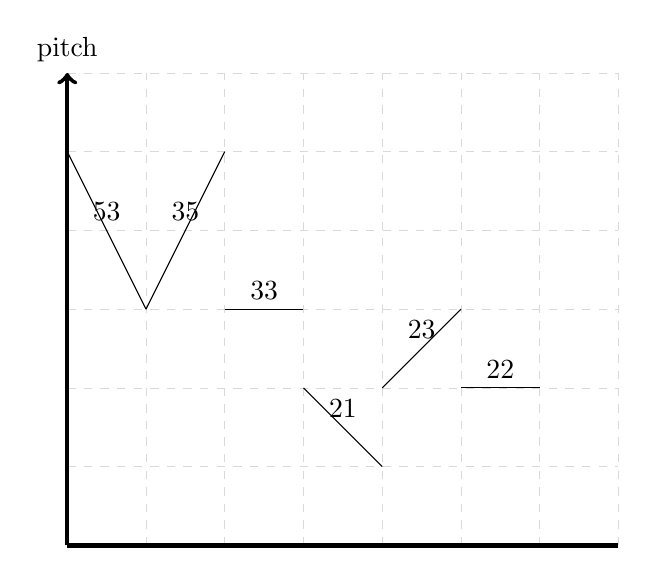
\begin{tikzpicture}
\draw [help lines, color=gray!30, dashed] (0, 0) grid (7, 6);
\draw [->, ultra thick] (0, 0) -- (0, 6) node [above]{pitch};
\draw [ultra thick] (0, 0) -- (7, 0);
\draw (0, 5) -- node [above]{53} (1, 3);
\draw (1, 3) -- node [above]{35} (2, 5);
\draw (2, 3) -- node [above]{33} (3, 3);
\draw (3, 2) -- node [above]{21} (4, 1);
\draw (4, 2) -- node [above]{23} (5, 3);
\draw (5, 2) -- node [above]{22} (6, 2);
\end{tikzpicture}

This is the way Cantonese themselves recite tones. You will note that the high level tone is not recieted traditionally. There are historical reasons for this which we won't go into here.

\end{minipage}

\begin{minipage}{\linewidth}

In a few words the consonants \underline{m} and \underline{ng} occur as vowels, and in this cases the diacritics are places above the \underline{n} of \underline{ng} and the \underline{m}.

\audioTag{A}{16:52}

\renewcommand{\arraystretch}{2}
\begin{tabularx}{\linewidth}{l l l}
    \jping{m4} & m̀h & not \\
    \jping{ng5} & ńgh & five \\
\end{tabularx}
\renewcommand{\arraystretch}{1}

\end{minipage}

%%%%%%%%%%%%%%%%%%%%%%%%%%%%%%%%%%%%%%%%
\begin{minipage}{\linewidth}

\paragraph{Tones in Sequence}

\underline{Tone Sandhi}. Changes in the basic sound of tones when syllables are spoken in sequence is called tone sandhi. The high falling tone in Cantonese undergoes tone sandhi in certain position, as follows:

\audioTag{A}{17:03}

1. When high falling tones occur in succession without intervening pause, all but the final ones are pronounced as high level:

Ex: hf + hf becomes hl + hf

\renewcommand{\arraystretch}{2}
\begin{tabularx}{\linewidth}{X X X}
roast pig (roast pork) & \dtext{燒豬}{siu7zyu7} & \dtext{燒豬}{siu1zyu7} \\
hurt wind (to catch cold) & \dtext{傷風}{soeng7fung7} & \dtext{傷風}{soeng1fung7} \\
hurt wind tim! (hurt wind!), caught cold! & \dtext{傷風添}{soeng7fung7tim7} & \dtext{傷風添}{soeng1fung1tim7} \\
\end{tabularx}
\renewcommand{\arraystretch}{1}

\audioTag{A}{17:43}

2. When a high falling tone occurs before a high level tone without intervening pause, it is pronounced as high level.

Ex: hf + hl becomes hl + hl

\renewcommand{\arraystretch}{2}
\begin{tabularx}{\linewidth}{X X X}
rent house (to rent a house) & \dtext{租屋}{zou7uk1} & \dtext{租屋}{zou1uk1} \\
west meal (western food) & \dtext{西餐}{sai7caan1} & \dtext{西餐}{sai1caan1} \\
\end{tabularx}
\renewcommand{\arraystretch}{1}

In this book high falling tone has been written high level only when the tone sandhi is within word boundaries. For separate words, the high falling will be marked with its usual diacritic.

\renewcommand{\arraystretch}{2}
\begin{tabularx}{\linewidth}{X X X}
first born (man, teacher, Mr.) & \dtext{先生}{sin7saang7} & \dtext{先生}{sin1saang7} \\
Cheung Mr. (Mr. Cheung) & \dtext{張生}{zoeng7saang7} & \dtext{張生}{zoeng7saang7} \\
\end{tabularx}
\renewcommand{\arraystretch}{1}

\end{minipage}

%%%%%%%%%%%%%%%%%%%%%%%%%%%%%%%%%%%%%%%%
\paragraph{Tones not 'sung'}

That Cantonese is a tone language does not mean that sentences in it are sung as you would sign a medical phrase. Music has sustained notes and strict rhythmic scheme, the spoken language does not. At first you may feel that Cantonese sounds sing-song, but practice will bring familiarity and soon it will sound natural to you.